% --------------------------- %
% Bakery Start
% --------------------------- %
\section{\textbf{Bakery Test}}
%%%%%%%%%%%%%%%%%%%%%%%%%%%%%%%%%%
\subsection{Particular Case}
\par
In this experiment, we are dealing with the problem of mutual exclusion with a
number of participants $>2$.
\par
We have already seen that Peterson Algorithm works for two threads. It garantees
mutual exclusion and is starvation free. Therefore, the algorithm is deadlock
free. Now let us focus in an algorithm that can be used to coordinate more
threads.
\par
%%%%%%%%%%%%%%%%%%%%%%%%%%%%%%%%%%
\subsection{Solution}
\par
The algorithm that we will play with is called Bakery. Its name comes from the
fact that it is similar to the protocol used in bakeries where one enters the
store and picks a number that indicates the order in which each client will be
attended. 
\par
In the algorithm, the fact of entering the store is done by setting a flag.
After that, the thread calculates the next number in the machine. 
\par
The algorithm then chooses the next number to be attended. When that happens,
the thread is allowed to enter the critical section.
\par
One thing that we ougth to mention is that threads can have the same number
assigned. If that is the case, the next in the line is decided using a
lexicographical ordering of the threads ids.
%%%%%%%%%%%%%%%%%%%%%%%%%%%%%%%%%%
\subsection{Experiment Description}
\par
Now let us explain how the experiments work. In this case we have 8 threads
increasing a counter from 0 to 1024. Each thread will increase the counter 128
times. At the end, the counter must remain in 1024. If that is not the case,
then there is a problem with the mutual exclusion.
\par
These are the details of the system we used to run the experiments:
\begin{itemize}
\item Processor: Intel Core i5 @2.5 GHz. 2 Cores.
\item L2 Cache per Core: 256 KB
\item L3 Cache: 3 MB
\item System Memory: 16 GB
\end{itemize}
%%%%%%%%%%%%%%%%%%%%%%%%%%%%%%%%%%
\subsection{Sample Results}
Figure \ref{fig:bakery00} and \ref{fig:bakery01} shows the output that we observed in the netbeans window:
\par
\begin{figure}[h]
  \centering
  \includegraphics[width=13cm]{Bakery00.png}
  \caption{Output of the junit test}
  \label{fig:bakery00}
\end{figure}
\par
\begin{figure}[h]
  \centering
  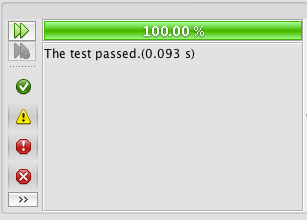
\includegraphics[width=5cm]{Bakery01.png}
  \caption{The Bakery test passed}
  \label{fig:bakery01}
\end{figure}
%%%%%%%%%%%%%%%%%%%%%%%%%%%%%%%%%%
\subsection{Interpretation}
\par
The results in the proposed system were all OK. In all cases, the  8 threads were
able to cooperate to increase the counter to 1024.
%%%%%%%%%%%%%%%%%%%%%%%%%%%%%%%%%%
% --------------------------- %
% Bakery End
% --------------------------- %
